% ============================================================
% HSBI Beamer — ISLP Lecture Series — IMPROVED EDITION
% Chapter 5: Resampling Methods
% ============================================================
\documentclass[aspectratio=169,11pt]{beamer}
\usepackage[utf8]{inputenc}\usepackage[T1]{fontenc}\usepackage[english]{babel}
\usepackage{graphicx}\usepackage{booktabs}\usepackage{amsmath,amssymb,amsfonts}
\usepackage{mathtools}\usepackage{hyperref}\usepackage{xcolor}
\usepackage{verbatim}\usepackage{alltt}
\usepackage{tikz}\usetikzlibrary{calc,arrows.meta,positioning,shapes}
\usepackage{tcolorbox}\tcbuselibrary{skins}

\usetheme{Madrid}\usecolortheme{default}
\setbeamertemplate{navigation symbols}{}
\setbeamertemplate{footline}[frame number]
\setbeamertemplate{blocks}[rounded][shadow=false]
\setbeamertemplate{headline}{%
  \leavevmode\hbox{%
    \begin{beamercolorbox}[wd=\paperwidth,ht=2.2ex,dp=0.9ex]{section in head/foot}%
      {\fontsize{4.6}{5.2}\selectfont%
       \insertsectionnavigationhorizontal{\paperwidth}{}{\hskip0pt plus1filll}}%
    \end{beamercolorbox}}%
}
\setbeamerfont{section in head/foot}{size=\tiny}
\setbeamerfont{palette primary}{size=\tiny}
\setbeamerfont{palette tertiary}{size=\tiny}
\setbeamerfont{section in toc}{size=\footnotesize}

\usepackage{listings}
\definecolor{pyKw}{RGB}{0,0,180}\definecolor{pyStr}{RGB}{20,120,40}
\definecolor{pyCom}{RGB}{120,120,120}\definecolor{accent}{RGB}{38,70,140}
\definecolor{cvtrain}{RGB}{38,70,140}\definecolor{cvtest}{RGB}{224,130,20}
\definecolor{cvgreen}{RGB}{46,125,50}\definecolor{cvred}{RGB}{198,40,40}
\lstdefinestyle{Pystyle}{language=Python,basicstyle=\ttfamily\footnotesize,
  keywordstyle=\color{pyKw}\bfseries,commentstyle=\color{pyCom}\itshape,
  stringstyle=\color{pyStr},showstringspaces=false,upquote=true,
  columns=fullflexible,breaklines=true,literate={~}{{$\sim$}}1}
\lstset{style=Pystyle}

\usepackage{etoolbox}
\makeatletter
\patchcmd{\beamer@sectionintoc}{\vskip1.5em}{\vskip.6em}{\typeout{TOCPATCH-OK}}{\typeout{TOCPATCH-FAIL}}
\makeatother

\AtBeginSection[]{\begin{frame}{Outline}\footnotesize
  \tableofcontents[currentsection,sectionstyle=show/shaded,subsectionstyle=show/show/hide]
\end{frame}}

\newcommand{\islpsource}[1]{%
  \vfill\hfill{\tiny\itshape\color{gray}Source: #1 \textemdash{} ISLP, James et al.\ (2023).}\par
}

\newtcolorbox{takeaway}[1][Takeaway]{enhanced,colback=green!4,colframe=green!50!black,
  boxrule=0pt,leftrule=2.5pt,arc=2pt,fonttitle=\bfseries,title=#1,
  left=2mm,right=2mm,top=1mm,bottom=1mm}
\newtcolorbox{numexample}[1][Worked example]{enhanced,colback=orange!4,colframe=orange!70!black,
  boxrule=0pt,leftrule=2.5pt,arc=2pt,fonttitle=\bfseries,title=#1,
  left=2mm,right=2mm,top=1mm,bottom=1mm}
\newtcolorbox{readme}[1][How to read this]{enhanced,colback=blue!4,colframe=accent,
  boxrule=0pt,leftrule=2.5pt,arc=2pt,fonttitle=\bfseries,title=#1,
  left=2mm,right=2mm,top=1mm,bottom=1mm}

\title{Quantitative Research Methods}
\subtitle{Chapter 5: Resampling Methods}
\author{Prof.\ Dr.\ Christoph Weisser}\institute{HSBI}
\date{Summer Semester 2026}\graphicspath{{images/}}

\newtcolorbox{exercise}[1][Exercise]{enhanced, fontupper=\footnotesize, colback=purple!4, colframe=purple!55!black, boxrule=0pt, leftrule=2.5pt, arc=2pt, fonttitle=\bfseries, title=#1, left=2mm, right=2mm, top=1mm, bottom=1mm}
\newtcolorbox{solutionbox}[1][Solution]{enhanced, fontupper=\footnotesize, colback=teal!5, colframe=teal!55!black, boxrule=0pt, leftrule=2.5pt, arc=2pt, fonttitle=\bfseries, title=#1, left=2mm, right=2mm, top=1mm, bottom=1mm}
\newtcolorbox{longexercise}[1][Extended exercise (15 min)]{enhanced, fontupper=\footnotesize, colback=violet!6, colframe=violet!55!black, boxrule=0pt, leftrule=3pt, arc=2pt, fonttitle=\bfseries, title=#1, left=2mm, right=2mm, top=1mm, bottom=1mm}

% Reclaim ~2pt of body height (custom nav headline makes full slides tip over by ~1.83pt)
\addtobeamertemplate{frametitle}{}{\vspace{-2pt}}

\newtcolorbox{labnote}[1][Run this live in the lab notebook]{enhanced, fontupper=\footnotesize, colback=cyan!7, colframe=cyan!45!black, boxrule=0pt, leftrule=3pt, arc=2pt, fonttitle=\bfseries, title=#1, left=2mm, right=2mm, top=1mm, bottom=1mm}

\begin{document}
\begin{frame}[plain]\titlepage\end{frame}

\begin{frame}{The course at a glance}
  \footnotesize
  \begin{center}
  \begin{tabular}{@{}c r l@{}}
    & \textbf{Lecture} & \textbf{Topic}\\
    \midrule
     & 1 & Ch.\ 1 + 2 --- Introduction; what is statistical learning \\
     & 2 & Ch.\ 2 --- Accuracy, bias--variance, Bayes classifier, KNN \\
     & 3--4 & Ch.\ 3 --- Linear regression (estimation, inference, diagnostics) \\
     & 5--6 & Ch.\ 4 --- Classification (logistic, LDA/QDA, naive Bayes, ROC) \\
    $\blacktriangleright$ & \textbf{7} & \textbf{Ch.\ 5 --- Resampling (validation, CV, bootstrap)} \\
     & 8 & Ch.\ 6 --- Model selection and regularisation (ridge, lasso) \\
     & 9 & Ch.\ 7 --- Moving beyond linearity (splines, GAMs) \\
     & 10 & Ch.\ 8 --- Tree-based methods (trees, forests, boosting) \\
     & 11 & Ch.\ 10 --- Deep learning (MLPs, CNNs, training) \\
     & 12 & Ch.\ 13 --- Multiple testing (FWER, FDR) \\
  \end{tabular}
  \end{center}
  \vspace{2pt}
  {\scriptsize Twelve sessions of 180 minutes. $\blacktriangleright$ marks today's chapter. Short exercises every $\sim$20 min; extended exercises every $\sim$45 min; each chapter has a companion lab notebook.}
\end{frame}


\begin{frame}{Contents}\small
  \tableofcontents[hideallsubsections]
\end{frame}

\begin{frame}{Notation in this chapter}
  \footnotesize
  \begin{center}
  \begin{tabular}{@{}ll@{}}
    \toprule
    \textbf{Symbol} & \textbf{Meaning} \\
    \midrule
    $e_i^2$ & Squared prediction error for held-out observation $i$ \\
    $\mathrm{CV}_{(n)}$ & LOOCV estimate of the test MSE ($n$ single-point folds) \\
    $h_i$ & Leverage of observation $i$ (one-fit OLS shortcut) \\
    $\mathrm{MSE}_j$ & Held-out mean squared error of fold $j$ \\
    $\mathrm{CV}_{(k)}$ & $k$-fold CV estimate: average of the $k$ fold errors \\
    $I(y_i \ne \hat y_i)$ & $0/1$ indicator loss used for classification CV \\
    $B$ & Number of bootstrap replications \\
    $\mathbf{Z}^{*b}$ & $b$-th bootstrap sample: $n$ rows drawn with replacement \\
    $\hat\alpha^{*b}$ & Statistic $\hat\alpha$ recomputed on $\mathbf{Z}^{*b}$ \\
    $\widehat{\mathrm{SE}}(\hat\alpha)$ & Bootstrap standard error: SD of the $B$ replicates \\
    \bottomrule
  \end{tabular}
  \end{center}
\end{frame}

\begin{frame}{Sources and references}
  \begin{block}{Primary textbook}
    James, G., Witten, D., Hastie, T., Tibshirani, R., \& Taylor, J.\ (2023).
    \emph{An Introduction to Statistical Learning, with Applications in
    Python.} Springer.
  \end{block}
  \begin{block}{About these slides}
    Each procedure is introduced with motivation, intuition, formal
    definition, and a worked example. Slide titles are descriptive;
    formulas are read symbol-by-symbol.
  \end{block}
\end{frame}

\begin{frame}{Learning objectives for this chapter}
  By the end of this chapter you will be able to:
  \begin{itemize}
    \item \textbf{Apply} the validation-set approach and articulate
          its weaknesses.
    \item \textbf{Compute} leave-one-out (LOOCV) and $k$-fold
          cross-validation test-error estimates.
    \item \textbf{Reason} about the bias--variance trade-off
          \emph{within} the cross-validation procedure itself.
    \item \textbf{Use} the bootstrap to obtain standard errors and
          confidence intervals when no closed-form formula exists.
    \item \textbf{Avoid} the common resampling pitfalls (information
          leakage, naive time-series folds, group-ignoring splits).
  \end{itemize}
\end{frame}


\begin{frame}{Roadmap of this chapter}
  \begin{takeaway}[Two big ideas and four procedures]
    \begin{itemize}
      \item \textbf{Cross-validation} for estimating test error:
            validation set, LOOCV, $k$-fold.
      \item \textbf{The bootstrap} for estimating standard errors and
            confidence intervals.
    \end{itemize}
  \end{takeaway}
  Why these matter: they are the practical workhorses you will use in
  every subsequent chapter to tune hyperparameters and report
  uncertainty.
\end{frame}

% ============================================================
\section{Why this chapter matters}
% ============================================================

\begin{frame}{The most important question in machine learning}
  Every model needs an honest answer to one question:
  \begin{takeaway}[The single most-asked question]
    \emph{``How well will my model perform on data it has not seen?''}
  \end{takeaway}
  Without an answer to this question, every other claim about a model
  is unfalsifiable.
\end{frame}

\begin{frame}{Why training error is the wrong answer}
  The model has been bent to fit the training points; the training
  error therefore overestimates how well the model would do on new
  data --- often dramatically.
  \begin{alertblock}{Training error is not test error}
    A flexible model can drive training error to zero while having
    arbitrarily bad test error. This is exactly the overfitting
    pathology of Chapter 2.
  \end{alertblock}
  \begin{takeaway}
    What we really want is the \emph{test} error. But how do we
    estimate it without an external test set? That is what this
    chapter is about.
  \end{takeaway}
\end{frame}

\begin{frame}{Two big ideas in this chapter}
  \begin{columns}[T]
    \begin{column}{0.48\textwidth}
      \begin{block}{Cross-validation}
        Repeatedly hold part of the data out, fit on the rest, score
        on the held-out part. Average the scores.
      \end{block}
      Used to estimate \textbf{test error}.
    \end{column}
    \begin{column}{0.48\textwidth}
      \begin{block}{The bootstrap}
        Sample \emph{with replacement} from the data many times,
        recompute the statistic each time, look at the spread.
      \end{block}
      Used to estimate \textbf{standard errors / confidence
      intervals}.
    \end{column}
  \end{columns}
  \begin{readme}[Which question does each answer?]
    Cross-validation answers \emph{``how accurate is my model?''};
    the bootstrap answers \emph{``how uncertain is my estimate?''} ---
    two different jobs, two different tools.
  \end{readme}
\end{frame}


% ============================================================
\section{Validation Set}
% ============================================================

\begin{frame}{The validation-set approach: split once, score once}
  The simplest possible resampling estimator: one random hold-out.
  \begin{center}
  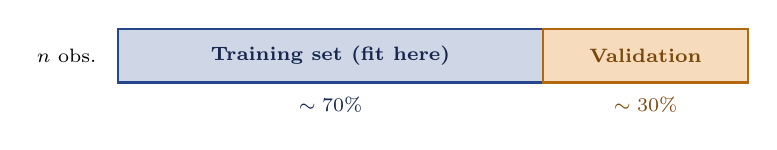
\begin{tikzpicture}
    \node[font=\scriptsize,anchor=east] at (-0.15,0) {$n$ obs.};
    \fill[cvtrain!22,draw=cvtrain,line width=0.9pt] (0,-0.34) rectangle (5.4,0.34);
    \fill[cvtest!28,draw=cvtest!80!black,line width=0.9pt] (5.4,-0.34) rectangle (8.0,0.34);
    \node[font=\scriptsize\bfseries,text=cvtrain!55!black] at (2.7,0) {Training set (fit here)};
    \node[font=\scriptsize\bfseries,text=cvtest!55!black] at (6.7,0) {Validation};
    \node[font=\scriptsize,anchor=north,text=cvtrain!55!black] at (2.7,-0.4) {$\sim70\%$};
    \node[font=\scriptsize,anchor=north,text=cvtest!55!black] at (6.7,-0.4) {$\sim30\%$};
  \end{tikzpicture}
  \end{center}
  \begin{block}{Recipe}
    \begin{enumerate}
      \item Randomly split the data into a training set and a
            validation (or hold-out) set --- typically 50/50 or 70/30.
      \item Fit the model on the training set; score it on the
            validation set.
    \end{enumerate}
  \end{block}
  \begin{readme}
    The validation MSE estimates the test MSE of a model trained on
    only $n_\mathrm{train}$ observations --- fewer than the full sample.
  \end{readme}
\end{frame}

\begin{frame}{Validation set: pros and cons}
  \begin{columns}[T]
    \begin{column}{0.48\textwidth}
      \textbf{Pros}
      \begin{itemize}
        \item Conceptually simple.
        \item Very fast --- one fit.
        \item Easy to explain.
      \end{itemize}
    \end{column}
    \begin{column}{0.48\textwidth}
      \textbf{Cons}
      \begin{itemize}
        \item Estimate is highly variable across random splits.
        \item Uses only part of the data for fitting --- tends to
              \emph{over}estimate test error.
      \end{itemize}
    \end{column}
  \end{columns}
  \begin{takeaway}
    Both weaknesses stem from using a \emph{single} split of only
    \emph{part} of the data. Averaging over several splits ---
    cross-validation --- attacks both at once.
  \end{takeaway}
\end{frame}

\begin{frame}{Validation across splits: how erratic is it?}
  \begin{center}
    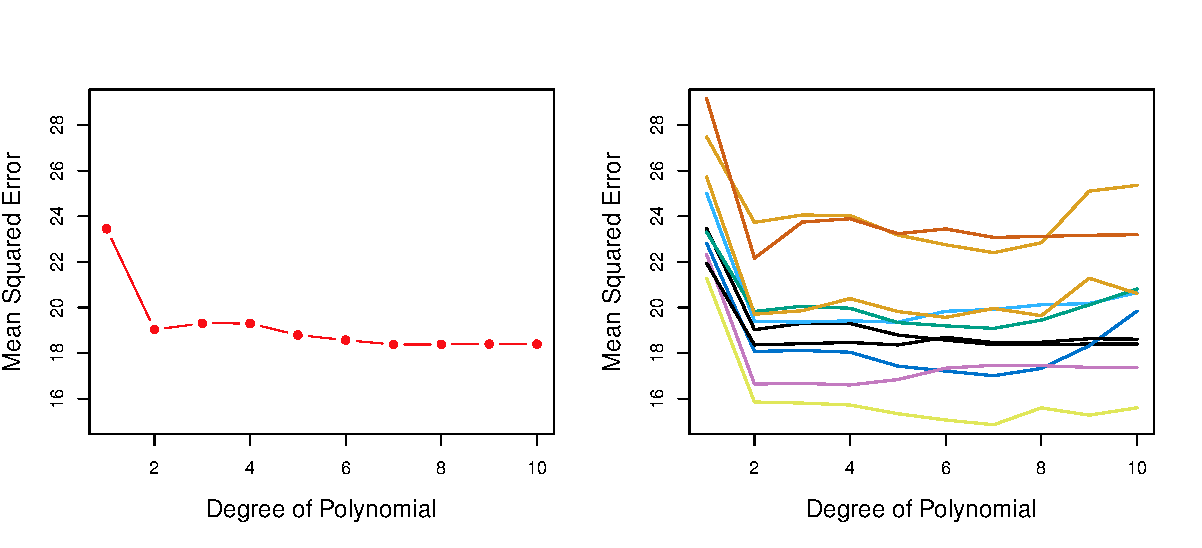
\includegraphics[width=0.92\textwidth,height=0.62\textheight,keepaspectratio]{5_2.pdf}
  \end{center}
  Multiple repetitions on the same data, with different random splits,
  produce visibly different validation curves --- and sometimes
  different ``optimal'' degrees.
  \islpsource{Figure 5.2}
\end{frame}

\begin{frame}{Exercise 5.1 --- Drawbacks of the Validation Set [Concept]}
  \begin{exercise}
    A colleague splits a data set of $n = 400$ observations once, at
    random, into a $50/50$ training/validation split, fits a model, and
    reports the validation MSE as ``the'' test error.
    \begin{enumerate}
      \item Name the \textbf{two} principal drawbacks of this
            validation-set approach.
      \item Explain why re-running the split with a different random seed
            can change which polynomial degree looks ``best''.
      \item Suggest one concrete change to the procedure that reduces
            both problems, and say why.
    \end{enumerate}
  \end{exercise}
\end{frame}

\begin{frame}{Solution --- Exercise 5.1}
  \begin{solutionbox}
    \textbf{(1) Two drawbacks.}
    \begin{itemize}
      \item \emph{High variability.} The estimate depends on the one
            random split. Different splits give visibly different
            validation MSEs, so the number is not reproducible.
      \item \emph{Pessimistic bias (fewer training observations).} Only
            half the data ($n_\mathrm{train} = 200$) is used to fit.
            Statistical methods generally perform worse with less
            training data, so the validation MSE tends to
            \emph{overestimate} the test error of the model that would
            be fit on all $400$ observations.
    \end{itemize}
    \textbf{(2) Why the ``best'' degree changes.}
    With only $200$ points in training and $200$ in validation, the
    validation curve is noisy. The differences between competing degrees
    are often smaller than that noise, so the argmin of the validation
    curve jumps between seeds --- exactly the erratic behaviour shown in
    Figure~5.2.

    \textbf{(3) A concrete fix.}
    Use $k$-fold cross-validation (e.g.\ $k = 10$) instead of a single
    split. Averaging over $k$ folds \emph{reduces variance} (the
    estimate no longer hinges on one split), and each fit now uses
    $\tfrac{k-1}{k}n = 360$ observations, which \emph{reduces the
    pessimistic bias}. Both drawbacks improve simultaneously.
  \end{solutionbox}
\end{frame}


% ============================================================
\section{LOOCV}
% ============================================================

\begin{frame}{Leave-one-out CV: take the validation idea to the limit}
  Make the validation set as small as possible: one observation.
  \begin{block}{LOOCV recipe}
    For $i = 1, \ldots, n$:
    \begin{enumerate}
      \item Train on all $n - 1$ observations except $i$.
      \item Predict for $i$; record the squared error $e_i^2$.
    \end{enumerate}
    LOOCV estimate of test MSE:
    \[
      \boxed{\;\mathrm{CV}_{(n)} = \tfrac{1}{n}\sum_{i=1}^n e_i^2.\;}
    \]
  \end{block}
\end{frame}

\begin{frame}{LOOCV as the $n$-fold limit (native diagram)}
  \begin{center}
  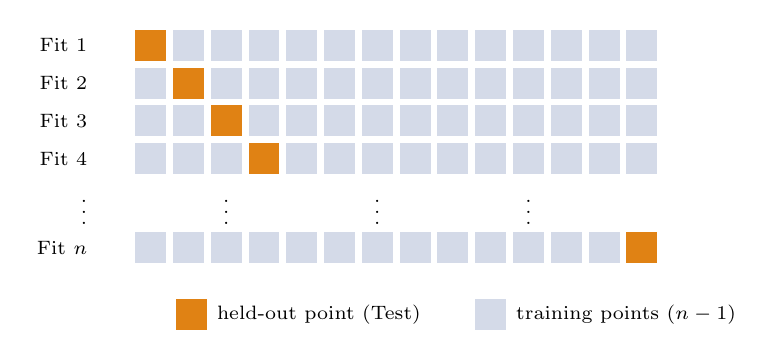
\begin{tikzpicture}
    \tikzset{ob/.style={draw=white,line width=0.8pt,minimum width=0.42cm,minimum height=0.42cm,inner sep=0pt,anchor=center}}
    \foreach \r in {1,...,4}{
      \node[font=\scriptsize,anchor=east] at (0.7,{-\r*0.48}) {Fit \r};
      \foreach \c in {1,...,14}{
        \ifnum\c=\r
          \node[ob,fill=cvtest] at ({\c*0.48+0.9},{-\r*0.48}) {};
        \else
          \node[ob,fill=cvtrain!20] at ({\c*0.48+0.9},{-\r*0.48}) {};
        \fi
      }
    }
    \node[font=\scriptsize,anchor=east] at (0.7,-2.5) {$\vdots$};
    \foreach \c in {3,7,11}{ \node[font=\scriptsize] at ({\c*0.48+0.9},-2.5) {$\vdots$}; }
    \node[font=\scriptsize,anchor=east] at (0.7,{-3.05}) {Fit $n$};
    \foreach \c in {1,...,14}{
      \ifnum\c=14
        \node[ob,fill=cvtest] at ({\c*0.48+0.9},{-3.05}) {};
      \else
        \node[ob,fill=cvtrain!20] at ({\c*0.48+0.9},{-3.05}) {};
      \fi
    }
    \node[ob,fill=cvtest] at (1.9,-3.9) {}; \node[anchor=west,font=\scriptsize] at (2.1,-3.9) {held-out point (Test)};
    \node[ob,fill=cvtrain!20] at (5.7,-3.9) {}; \node[anchor=west,font=\scriptsize] at (5.9,-3.9) {training points ($n-1$)};
  \end{tikzpicture}
  \end{center}
  \begin{takeaway}
    LOOCV is $k$-fold with $k=n$: each observation is held out exactly once, giving $n$ fits and $\mathrm{CV}_{(n)}=\tfrac1n\sum_{i=1}^n e_i^2$. Lowest bias, but $n$ fits --- use the OLS leverage shortcut when it applies.
  \end{takeaway}
\end{frame}

\begin{frame}{Reading the LOOCV formula}
  \begin{readme}
    \begin{itemize}
      \item Each $e_i^2$ is computed using a model that did
            \emph{not} see observation $i$ during training.
      \item Averaging $n$ such squared prediction errors gives an
            (almost) unbiased estimate of the test MSE.
      \item Because every fit uses $n - 1$ training points, the bias
            is very small.
    \end{itemize}
  \end{readme}
  \begin{takeaway}[Pros]
    Uses (almost) all data for training; deterministic --- no random
    splits; symmetric --- every observation gets the same treatment.
  \end{takeaway}
\end{frame}

\begin{frame}{LOOCV's hidden cost}
  \begin{alertblock}{Computational cost}
    Naive LOOCV requires fitting the model $n$ times. With $n = 10^4$
    and a complex model, this is impractical.
  \end{alertblock}
  \begin{takeaway}[The OLS shortcut]
    For \emph{ordinary least squares} (and ridge regression), there
    is a one-fit shortcut using the leverage statistic.
  \end{takeaway}
\end{frame}

\begin{frame}{The OLS LOOCV shortcut}
  For OLS regression specifically:
  \begin{block}{LOOCV formula for OLS}
    \[
      \mathrm{CV}_{(n)} = \frac{1}{n}\sum_{i=1}^n
        \left(\frac{y_i - \hat y_i}{1 - h_i}\right)^2,
    \]
    where $h_i$ is the leverage of observation $i$ (the $i$-th
    diagonal of the hat matrix, Ch.~3).
  \end{block}
  \begin{readme}
    The denominator $1 - h_i$ corrects for the influence each point
    has on its own fitted value. High-leverage points get a stronger
    correction. One fit + the diagonal of $\mathbf{H}$ replaces $n$
    fits.
  \end{readme}
\end{frame}

\begin{frame}{Exercise 5.2 --- LOOCV Fits and the Leverage Shortcut [Math]}
  \begin{exercise}
    Consider a data set with $n = 500$ observations.
    \begin{enumerate}
      \item How many separate model fits does \emph{naive} LOOCV
            require? How many for $10$-fold CV?
      \item State the OLS leverage shortcut for $\mathrm{CV}_{(n)}$ and
            explain how many full model fits it needs.
      \item For a simple linear regression with $n = 4$ points, one
            observation has residual $y_i - \hat y_i = 2.0$ and leverage
            $h_i = 0.5$. Compute this point's contribution
            $\bigl(\tfrac{y_i-\hat y_i}{1-h_i}\bigr)^2$ to the LOOCV sum
            and compare it with the naive squared residual $e_i^2$.
    \end{enumerate}
  \end{exercise}
\end{frame}

\begin{frame}{Solution --- Exercise 5.2 (1/2)}
  \begin{solutionbox}
    \textbf{(1) Number of fits.}
    Naive LOOCV leaves out one observation at a time and refits, so it
    requires $n = 500$ fits. $10$-fold CV refits once per fold, so it
    requires $10$ fits.

    \textbf{(2) The OLS shortcut.}
    For ordinary least squares,
    \[
      \mathrm{CV}_{(n)} = \frac{1}{n}\sum_{i=1}^n
        \left(\frac{y_i - \hat y_i}{1 - h_i}\right)^2 ,
    \]
    where $\hat y_i$ and the leverages $h_i$ (diagonal of the hat matrix
    $\mathbf{H} = \mathbf{X}(\mathbf{X}^\top\mathbf{X})^{-1}\mathbf{X}^\top$)
    come from a \emph{single} fit on the full data. So it needs only
    \textbf{one} fit instead of $n$ --- a dramatic saving.

    \emph{Why this works:} OLS is a linear smoother, so deleting
    observation $i$ changes its own fitted value in a way captured
    entirely by $h_i$; the $n$ leave-one-out residuals can therefore be
    recovered \emph{exactly} --- not approximately --- from one fit. No
    such identity exists for general nonlinear models.
  \end{solutionbox}
\end{frame}

\begin{frame}{Solution --- Exercise 5.2 (2/2)}
  \begin{solutionbox}
    \textbf{(3) Numerical contribution.}
    \[
      \left(\frac{y_i - \hat y_i}{1 - h_i}\right)^2
      = \left(\frac{2.0}{1 - 0.5}\right)^2
      = \left(\frac{2.0}{0.5}\right)^2
      = 4.0^2 = 16.0 .
    \]
    The naive squared residual is $e_i^2 = 2.0^2 = 4.0$. The shortcut
    inflates this high-leverage point's contribution by the factor
    $1/(1-h_i)^2 = 1/0.25 = 4$, correctly reflecting that a
    high-leverage point strongly pulls the fitted line toward itself, so
    its genuine leave-one-out error is much larger than the in-sample
    residual suggests.

    \emph{Interpretation.} The in-sample residual understates this
    point's out-of-sample error by a factor of $4$: remove the point and
    the fitted line springs back, so the prediction misses it far more
    badly than the training residual admits.

    \emph{Common mistake:} forgetting that $y_i - \hat y_i$ and $h_i$
    both come from the \emph{full-data} fit (no refitting is involved),
    or dividing by $1-h_i$ without squaring --- the correction factor on
    the \emph{squared} error is $1/(1-h_i)^2 = 4$, not $1/(1-h_i) = 2$.
  \end{solutionbox}
\end{frame}


% ============================================================
\section{$k$-Fold CV}
% ============================================================

\begin{frame}{$k$-fold CV: a practical compromise}
  Between the (variable) validation set and the (slow) LOOCV.
  \begin{block}{Recipe}
    \begin{enumerate}
      \item Split the data into $k$ roughly equal folds (typically
            $k = 5$ or $k = 10$).
      \item For each fold $j = 1, \ldots, k$: train on the other
            $k - 1$ folds, validate on fold $j$.
      \item Average the $k$ validation errors.
    \end{enumerate}
  \end{block}
  Every observation appears in the validation fold exactly once and
  in the training fold $k - 1$ times.
  \begin{takeaway}
    $k$-fold inherits LOOCV's near-full training sets \emph{and} the
    validation set's low cost: only $k$ fits, low bias, moderate
    variance.
  \end{takeaway}
\end{frame}

\begin{frame}{Visualising 5-fold CV}
  \begin{center}
    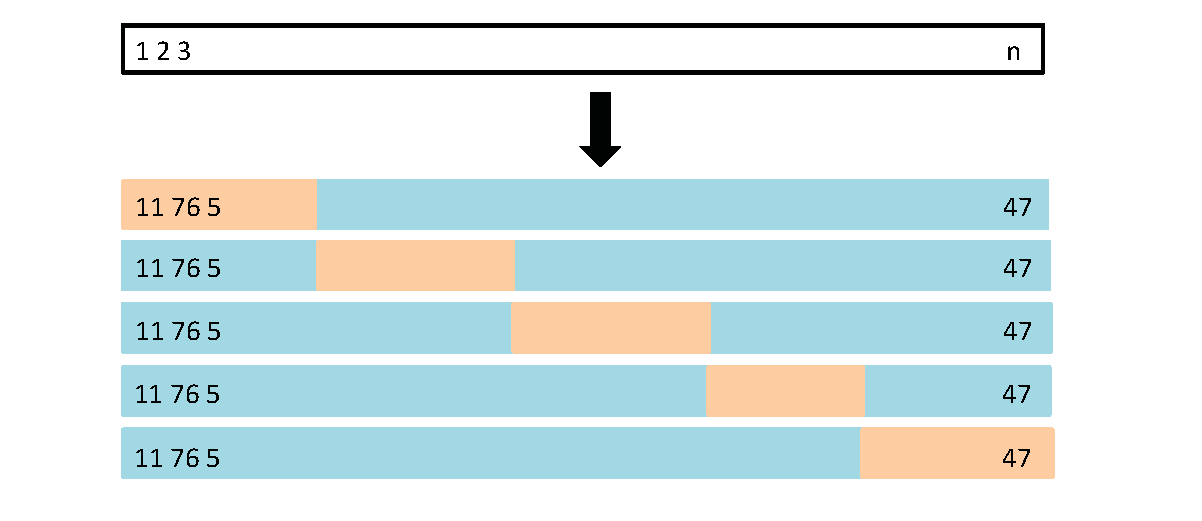
\includegraphics[width=0.95\textwidth,height=0.45\textheight,keepaspectratio]{5_5.pdf}
  \end{center}
  Each row is one of the five folds. Blue blocks are training, beige
  blocks are validation.
  \islpsource{Figure 5.5}
\end{frame}

\begin{frame}{$k$-fold cross-validation, step by step (native diagram)}
  \begin{center}
  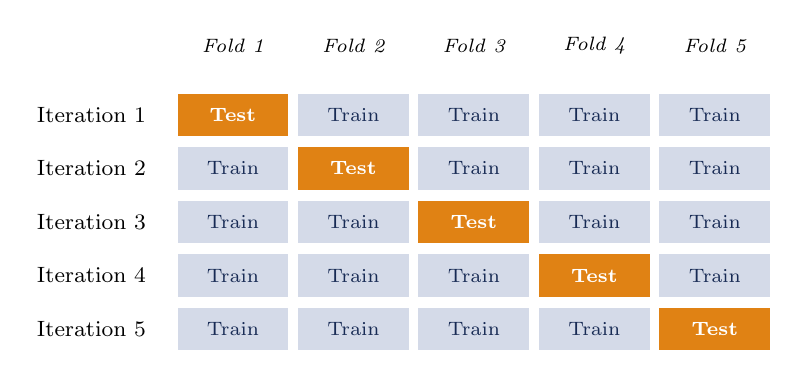
\begin{tikzpicture}
    \tikzset{cell/.style={draw=white,line width=1.2pt,minimum width=1.45cm,minimum height=0.58cm,anchor=center}}
    \foreach \c in {1,...,5}{ \node[font=\scriptsize\itshape] at ({\c*1.53},0.2) {Fold \c}; }
    \foreach \r in {1,...,5}{
      \node[font=\footnotesize,anchor=east] at (0.55,{-\r*0.68}) {Iteration \r};
      \foreach \c in {1,...,5}{
        \ifnum\c=\r
          \node[cell,fill=cvtest,text=white,font=\scriptsize\bfseries] at ({\c*1.53},{-\r*0.68}) {Test};
        \else
          \node[cell,fill=cvtrain!20,text=cvtrain!60!black,font=\scriptsize] at ({\c*1.53},{-\r*0.68}) {Train};
        \fi
      }
    }
  \end{tikzpicture}
  \end{center}
  \begin{takeaway}
    Each of the five folds serves as the test set exactly once (orange); the rest train the model. The estimate is the average of the five held-out errors: $\mathrm{CV}_{(5)}=\tfrac15\sum_{j=1}^{5}\mathrm{MSE}_j$.
  \end{takeaway}
\end{frame}

\begin{frame}{LOOCV vs.\ $k$-fold: the bias-variance trade-off}
  \begin{columns}[T]
    \begin{column}{0.48\textwidth}
      \begin{block}{LOOCV}
        \emph{Lowest bias} (training sets nearly the full size) but
        \emph{highest variance}: the $n$ training sets overlap
        enormously, so the $n$ errors are highly correlated.
      \end{block}
    \end{column}
    \begin{column}{0.48\textwidth}
      \begin{block}{5-fold CV}
        Slightly upward biased (smaller training sets) but
        \emph{much lower variance} because the $k$ training sets share
        less data.
      \end{block}
    \end{column}
  \end{columns}
  \begin{takeaway}[Practical recommendation]
    The $k = 10$ rule of thumb usually wins on mean-squared error of
    the test-error estimate. Use LOOCV only when the OLS shortcut
    applies or $n$ is tiny.
  \end{takeaway}
\end{frame}

\begin{frame}{Why $k \approx 10$ wins: visualising the trade-off}
  \begin{center}
    
\includegraphics[width=0.84\textwidth,height=0.52\textheight,keepaspectratio]{ch05_cv_bias_variance.png}
  \end{center}
  \begin{takeaway}
    More folds $\Rightarrow$ larger training sets (\emph{less bias}) but
    training sets that overlap more (\emph{more variance}). The total
    error of the estimate is smallest around $k = 5$--$10$ --- neither
    the single split ($k=2$) nor LOOCV ($k=n$).
  \end{takeaway}
\end{frame}

\begin{frame}{Cross-validation in practice: choosing the polynomial degree}
  \begin{center}
    
\includegraphics[width=0.82\textwidth,height=0.58\textheight,keepaspectratio]{ch05_cv_degree.png}
  \end{center}
  \begin{takeaway}
    On Auto (\texttt{mpg}$\sim$\texttt{poly(horsepower,d)}), LOOCV and 10-fold CV both drop sharply from degree 1 to 2 then stay flat --- CV points to a low-degree model.
  \end{takeaway}
\end{frame}

\begin{frame}{Cross-validation for classification}
  For a qualitative response, swap squared error for the $0/1$
  misclassification loss:
  \[
    \mathrm{CV}_{(n)} = \frac{1}{n}\sum_{i=1}^n
      I\bigl(y_i \ne \hat y_i^{(-i)}\bigr).
  \]
  \begin{readme}
    \begin{itemize}
      \item $I(\cdot)$ is the indicator: $1$ when the prediction is
            \emph{wrong}, $0$ when it is right.
      \item $\hat y_i^{(-i)}$ is the class predicted for $i$ by a model
            fit \emph{without} observation $i$.
      \item So $\mathrm{CV}_{(n)}$ is just the held-out error
            \emph{rate} --- the fraction of points misclassified.
    \end{itemize}
  \end{readme}
  \begin{takeaway}
    Same mechanics, different loss. For threshold-dependent metrics
    (sensitivity at fixed specificity), \emph{nest} the CV: tune the
    threshold inside, score the model outside.
  \end{takeaway}
\end{frame}

\begin{frame}{CV in action: KNN on a synthetic problem}
  \begin{center}
    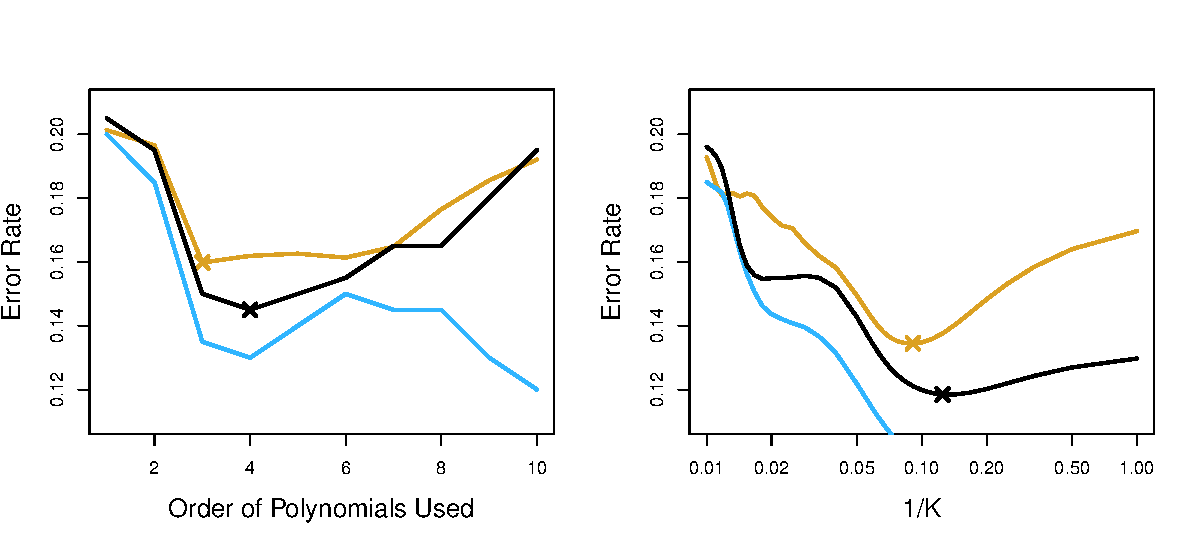
\includegraphics[width=0.85\textwidth,height=0.62\textheight,keepaspectratio]{5_8.pdf}
  \end{center}
  CV closely tracks the true test error --- justifying its use for
  hyperparameter selection.
  \islpsource{Figure 5.8}
\end{frame}

\begin{frame}{Three pitfalls that quietly invalidate CV}
  \begin{alertblock}{The classic CV mistakes}
    \begin{enumerate}
      \item \textbf{Information leakage.} Any preprocessing fit on the
            \emph{full} data and used inside CV (scaling, feature
            selection, imputation) corrupts the estimate. Always fit
            preprocessing inside the CV loop.
      \item \textbf{Time series.} Vanilla random folds destroy
            temporal order. Use rolling-origin or expanding-window CV.
      \item \textbf{Grouped data.} CV folds must respect groups
            (patients, customers) to avoid within-group leakage.
    \end{enumerate}
  \end{alertblock}
\end{frame}


\begin{frame}{Mini-check: cross-validation}
  \begin{readme}[Quick self-assessment]
    \begin{enumerate}
      \item Why does 10-fold CV usually beat LOOCV on mean-squared error
            of the test-error estimate?
      \item For a time series, why are random folds wrong?
      \item If you standardise predictors on the full data and then run
            CV, what is the consequence?
    \end{enumerate}
  \end{readme}
  \begin{takeaway}[Answers]
    1.\ The $n$ training sets in LOOCV overlap heavily, so the $n$ errors
        are correlated --- variance of the average is high.\quad
    2.\ They destroy temporal order; future leaks into training.\quad
    3.\ Information leakage: the test fold informed the standardisation.
  \end{takeaway}
\end{frame}

\begin{frame}{Exercise 5.3 --- $k$-Fold vs.\ LOOCV Trade-off [Concept]}
  \begin{exercise}
    \begin{enumerate}
      \item Place validation-set, $10$-fold CV, and LOOCV on the
            \emph{bias} axis and on the \emph{variance} axis of their
            test-error estimates. Justify each ranking in one sentence.
      \item Why are the $n$ error terms in LOOCV so highly correlated,
            and why does that inflate the variance of the average?
      \item Why is $k = 5$ or $k = 10$ the usual recommendation?
    \end{enumerate}
  \end{exercise}
\end{frame}

\begin{frame}{Solution --- Exercise 5.3}
  \begin{solutionbox}
    \textbf{(1) Bias and variance rankings.}
    \begin{itemize}
      \item \emph{Bias} (of the test-error estimate): validation set is
            \emph{highest} (trains on only $\sim n/2$); $10$-fold is
            intermediate (trains on $0.9n$); LOOCV is \emph{lowest}
            (trains on $n-1$, essentially the full sample).
      \item \emph{Variance}: LOOCV is \emph{highest}; $10$-fold is
            \emph{moderate}; the single validation set is also highly
            variable across splits. So on the bias--variance trade-off,
            $10$-fold sits in the sweet spot.
    \end{itemize}
    \textbf{(2) Correlated errors in LOOCV.}
    Any two LOOCV training sets share $n-2$ of their $n-1$ observations,
    so the $n$ fitted models are almost identical and their errors are
    highly positively correlated. The variance of an average of
    positively correlated terms (each with variance $\sigma^2$ and average
    pairwise correlation $\rho$),
    $\mathrm{Var}(\bar e) = \tfrac{1}{n}\sigma^2 +
    \tfrac{n-1}{n}\rho\,\sigma^2$, does not shrink toward zero when
    $\rho$ is large --- hence high variance. In $k$-fold with small $k$
    the training sets overlap less, so $\rho$ is smaller.

    \textbf{(3) Why $k = 5$ or $10$.}
    These values give training sets of $80$--$90\%$ of the data (small
    bias) while keeping the fold errors only moderately correlated
    (moderate variance), and they cost only $5$ or $10$ fits. Empirically
    they minimise the mean-squared error of the test-error estimate ---
    the best of both worlds.
  \end{solutionbox}
\end{frame}

\begin{frame}{Exercise 5.4 --- Computing a $k$-Fold CV Estimate [Math]}
  \begin{exercise}
    A $5$-fold cross-validation of a regression model produces the
    following per-fold mean squared errors:
    \[
      \mathrm{MSE}_1 = 10.2,\;
      \mathrm{MSE}_2 = 12.4,\;
      \mathrm{MSE}_3 = 9.6,\;
      \mathrm{MSE}_4 = 11.8,\;
      \mathrm{MSE}_5 = 10.0 .
    \]
    \begin{enumerate}
      \item Compute the $5$-fold CV error estimate $\mathrm{CV}_{(5)}$.
      \item Compute the standard deviation of the five fold errors and
            the standard error of the mean.
      \item If the folds have unequal sizes $n_j$, how should the
            average be modified?
    \end{enumerate}
  \end{exercise}
\end{frame}

\begin{frame}{Solution --- Exercise 5.4 (1/2)}
  \begin{solutionbox}
    \textbf{(1) CV estimate.}
    \[
      \mathrm{CV}_{(5)} = \frac{1}{5}\sum_{j=1}^{5}\mathrm{MSE}_j
      = \frac{10.2+12.4+9.6+11.8+10.0}{5}
      = \frac{54.0}{5} = 10.8 .
    \]
    \textbf{(2) Spread of the fold errors.}
    Deviations from the mean $10.8$ are
    $-0.6,\,1.6,\,-1.2,\,1.0,\,-0.8$; their squares sum to
    $0.36+2.56+1.44+1.00+0.64 = 6.0$. The sample standard deviation is
    \[
      s = \sqrt{\frac{6.0}{5-1}} = \sqrt{1.5} \approx 1.22 ,
    \]
    and the standard error of the mean is
    $s/\sqrt{5} \approx 1.22/2.236 \approx 0.55$.
    So $\mathrm{CV}_{(5)} \approx 10.8 \pm 0.55$.

    \emph{Interpretation.} The five folds agree to within about $5\%$
    of the estimate ($0.55/10.8$), so the CV number is stable; quoting
    $10.8$ \emph{with} its spread is what turns a point estimate into a
    defensible claim.
  \end{solutionbox}
\end{frame}

\begin{frame}{Solution --- Exercise 5.4 (2/2)}
  \begin{solutionbox}
    \textbf{(3) Unequal fold sizes.}
    Use a size-weighted average so every observation counts equally:
    \[
      \mathrm{CV}_{(k)} = \frac{1}{n}\sum_{j=1}^{k} n_j\,\mathrm{MSE}_j ,
      \qquad n = \sum_{j=1}^k n_j .
    \]
    With equal fold sizes this reduces to the simple mean in part (1).

    \emph{Why weight?} Fold $j$'s error is
    $\mathrm{MSE}_j = \tfrac{1}{n_j}\sum_{i \in \text{fold } j} e_i^2$,
    so $n_j\,\mathrm{MSE}_j$ restores the fold's \emph{total} squared
    error and dividing by $n$ yields exactly the mean of all $n$
    individual squared errors --- every observation counts once.

    \emph{Micro-example.} Folds of sizes $90$ and $110$ with
    $\mathrm{MSE} = 10$ and $12$: unweighted mean $11.0$, correct
    weighted value $\tfrac{90(10) + 110(12)}{200} = \tfrac{2220}{200}
    = 11.1$ --- the larger fold rightly counts more.

    \emph{Common mistake:} averaging fold MSEs unweighted when fold
    sizes differ; with equal folds the two coincide, which is why the
    slip often goes unnoticed.
  \end{solutionbox}
\end{frame}

\begin{frame}{Extended Exercise 5.1 --- LOOCV Shortcut vs.\ 5-Fold CV [Math]}
  \begin{longexercise}
    A simple linear regression (one predictor, so $p+1=2$ parameters) is
    fit by OLS to $n = 200$ observations, giving a training residual sum
    of squares $\mathrm{RSS} = \sum_i e_i^2 = 760$.
    \begin{enumerate}
      \item \textbf{Leverage shortcut, per point.} Three representative
            observations have (residual $e_i$, leverage $h_i$):
            $A=(1.0,\,0.02)$, $B=(3.0,\,0.30)$, $C=(-2.0,\,0.05)$.
            Compute each LOOCV contribution $\bigl(e_i/(1-h_i)\bigr)^2$
            and compare with the naive $e_i^2$.
      \item \textbf{Leverage shortcut, whole sample.} The average OLS
            leverage is $\bar h=(p+1)/n$. Using the approximation that
            all $h_i\approx\bar h$, estimate
            $\mathrm{CV}_{(n)}\approx \mathrm{MSE}_{\text{train}}/(1-\bar h)^2$.
      \item \textbf{5-fold CV.} A 5-fold run gives per-fold MSEs
            $4.0,\,4.4,\,3.8,\,4.6,\,4.2$. Compute $\mathrm{CV}_{(5)}$ and
            its standard error across folds.
      \item \textbf{Compare} the two estimates and their bias--variance
            properties. Which is cheaper \emph{here}, and why does that
            not usually hold?
    \end{enumerate}
  \end{longexercise}
\end{frame}

\begin{frame}{Solution --- Extended Exercise 5.1 (1/2)}
  \begin{solutionbox}
    \textbf{(1) Per-point leverage correction.}
    \[
      A:\ \Bigl(\tfrac{1.0}{0.98}\Bigr)^2\!=\!1.04,\quad
      B:\ \Bigl(\tfrac{3.0}{0.70}\Bigr)^2\!=\!18.37,\quad
      C:\ \Bigl(\tfrac{-2.0}{0.95}\Bigr)^2\!=\!4.43,
    \]
    versus the naive $e_i^2 = 1.0,\ 9.0,\ 4.0$. The correction factor
    $1/(1-h_i)^2$ equals $1.04,\ 2.04,\ 1.11$: the high-leverage point
    $B$ is inflated most, because it pulls the fit strongly toward
    itself, so its true leave-one-out error far exceeds the in-sample
    residual.

    \textbf{(2) Whole-sample shortcut.}
    $\bar h=(p+1)/n=2/200=0.01$ and
    $\mathrm{MSE}_{\text{train}}=\mathrm{RSS}/n=760/200=3.80$, hence
    \[
      \mathrm{CV}_{(n)}\approx\frac{3.80}{(1-0.01)^2}
      =\frac{3.80}{0.9801}\approx 3.88 .
    \]
    A single OLS fit plus the hat-matrix diagonal replaces $n=200$ fits.
    Note that $3.88$ sits just \emph{above}
    $\mathrm{MSE}_{\text{train}} = 3.80$: the $1/(1-\bar h)^2$ factor
    always inflates the training error, undoing its optimism.
  \end{solutionbox}
\end{frame}

\begin{frame}{Solution --- Extended Exercise 5.1 (2/2)}
  \begin{solutionbox}
    \textbf{(3) 5-fold estimate.}
    $\mathrm{CV}_{(5)}=\tfrac15(4.0+4.4+3.8+4.6+4.2)=\tfrac{21.0}{5}=4.20$.
    Deviations from $4.20$ are $-0.2,0.2,-0.4,0.4,0.0$; their squares sum
    to $0.40$, so $s=\sqrt{0.40/4}=\sqrt{0.1}\approx0.316$ and the
    standard error is $s/\sqrt5\approx0.14$: $\mathrm{CV}_{(5)}\approx
    4.20\pm0.14$.

    \textbf{(4) Comparison.} Both estimates target the same test MSE and
    agree closely ($3.88$ vs.\ $4.20$).
    \begin{itemize}
      \item \emph{Bias}: LOOCV trains on $199$ points (almost unbiased);
            5-fold trains on $160$, so it is slightly pessimistic ---
            consistent with $4.20>3.88$.
      \item \emph{Variance}: LOOCV averages $n$ highly correlated fits
            (higher variance); 5-fold averages $5$ weakly correlated
            fits (lower variance).
      \item \emph{Cost}: here LOOCV is \emph{cheaper} --- the leverage
            shortcut is one fit versus five. This reversal is special to
            OLS/ridge; for a general model LOOCV costs $n$ fits.
    \end{itemize}
    \emph{Common mistake:} reading $3.88 < 4.20$ as ``LOOCV is more
    accurate''. Both target the same test MSE; the gap mostly reflects
    5-fold's pessimistic bias (training on $160$ rather than $199$
    points), not a defect of either estimate.
  \end{solutionbox}
\end{frame}

% ============================================================
\section{The Bootstrap}
% ============================================================

\begin{frame}{Why we need the bootstrap}
  We often want the standard error or sampling distribution of a
  statistic $\hat\alpha$ for which no closed-form formula exists.
  \begin{takeaway}[The thought experiment]
    \emph{If only we could see many independent samples!} Then we
    could just compute $\hat\alpha$ on each sample and take the
    empirical SD.
  \end{takeaway}
  We don't have many samples --- we have one. The bootstrap is a
  trick to simulate ``many samples'' from the one we have.
\end{frame}

\begin{frame}{The bootstrap algorithm}
  \begin{block}{Recipe}
    \begin{enumerate}
      \item Draw $B$ bootstrap samples
            $\mathbf{Z}^{*1}, \ldots, \mathbf{Z}^{*B}$, each by
            sampling $n$ rows \emph{with replacement} from the data.
      \item Compute the statistic $\hat\alpha^{*b}$ on each.
      \item Estimate the standard error by (with $\bar\alpha^*=\tfrac1B\sum_b\hat\alpha^{*b}$ the mean of the replicates):
            \[
              \widehat{\mathrm{SE}}(\hat\alpha) =
              \sqrt{\frac{1}{B-1}\sum_{b=1}^B
                \bigl(\hat\alpha^{*b} - \bar\alpha^*\bigr)^2}.
            \]
      \item Build percentile $(1 - \alpha)$ confidence intervals as
            $[\hat\alpha^*_{\alpha/2}, \hat\alpha^*_{1-\alpha/2}]$.
    \end{enumerate}
  \end{block}
\end{frame}

\begin{frame}{The bootstrap, schematically (native diagram)}
  \begin{center}
  \resizebox{0.98\textwidth}{!}{%
  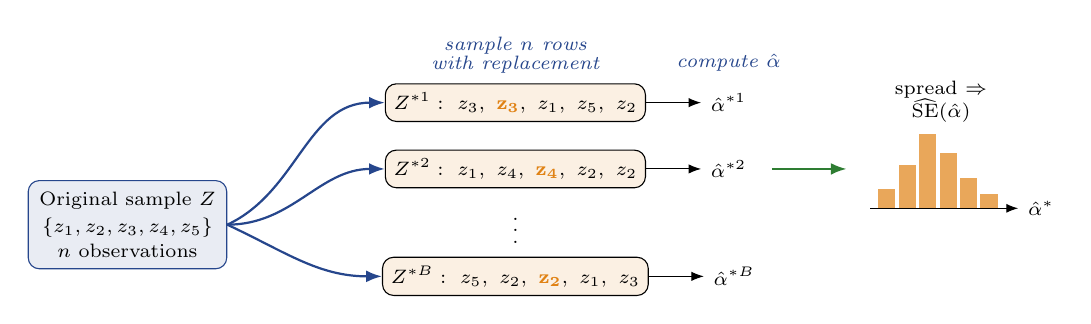
\begin{tikzpicture}[font=\scriptsize]
    \node[draw=cvtrain,fill=cvtrain!10,rounded corners,inner sep=4pt,align=center] (orig)
       {Original sample $Z$\\[2pt]$\{z_1,z_2,z_3,z_4,z_5\}$\\[1pt]$n$ observations};
    \node[draw,fill=cvtest!12,rounded corners,inner sep=3pt,align=left,right=2.0cm of orig,yshift=1.55cm] (b1)
       {$Z^{*1}:\ z_3,\ \textcolor{cvtest}{\mathbf{z_3}},\ z_1,\ z_5,\ z_2$};
    \node[draw,fill=cvtest!12,rounded corners,inner sep=3pt,align=left,below=3.5mm of b1] (b2)
       {$Z^{*2}:\ z_1,\ z_4,\ \textcolor{cvtest}{\mathbf{z_4}},\ z_2,\ z_2$};
    \node[below=0.5mm of b2] (bd) {$\vdots$};
    \node[draw,fill=cvtest!12,rounded corners,inner sep=3pt,align=left,below=0.5mm of bd] (bB)
       {$Z^{*B}:\ z_5,\ z_2,\ \textcolor{cvtest}{\mathbf{z_2}},\ z_1,\ z_3$};
    \draw[-{Latex[length=2mm]},cvtrain,thick] (orig.east) to[out=25,in=180] (b1.west);
    \draw[-{Latex[length=2mm]},cvtrain,thick] (orig.east) to[out=0,in=180] (b2.west);
    \draw[-{Latex[length=2mm]},cvtrain,thick] (orig.east) to[out=-25,in=180] (bB.west);
    \node[cvtrain,align=center,above=0mm of b1] {\itshape sample $n$ rows\\[-1pt]\itshape with replacement};
    \node[right=7mm of b1] (a1) {$\hat\alpha^{*1}$};
    \node[right=7mm of b2] (a2) {$\hat\alpha^{*2}$};
    \node[right=7mm of bB] (aB) {$\hat\alpha^{*B}$};
    \draw[-{Latex[length=1.6mm]}] (b1.east)--(a1.west);
    \draw[-{Latex[length=1.6mm]}] (b2.east)--(a2.west);
    \draw[-{Latex[length=1.6mm]}] (bB.east)--(aB.west);
    \node[above=0.4mm of a1,cvtrain,font=\scriptsize\itshape] {compute $\hat\alpha$};
    \draw[-{Latex[length=2mm]},cvgreen,thick] ($(a2.east)+(0.2,0)$) -- ($(a2.east)+(1.15,0)$);
    \begin{scope}[shift={($(a2.east)+(1.55cm,0)$)}]
       \foreach \x/\h in {0/0.25,0.26/0.55,0.52/0.95,0.78/0.7,1.04/0.38,1.30/0.18}{
          \fill[cvtest!70] (\x,-0.5) rectangle ({\x+0.22},{-0.5+\h});}
       \draw[-{Latex[length=1.5mm]}] (-0.1,-0.5)--(1.78,-0.5) node[right,font=\scriptsize]{$\hat\alpha^{*}$};
       \node[align=center,font=\scriptsize] at (0.8,0.85) {spread $\Rightarrow$\\[-1pt]$\widehat{\mathrm{SE}}(\hat\alpha)$};
    \end{scope}
  \end{tikzpicture}}
  \end{center}
  \begin{takeaway}
    Resample the rows \emph{with replacement} (note the repeated observations in orange), recompute $\hat\alpha$ on each of the $B$ samples, and read the standard error off the spread of the replicates.
  \end{takeaway}
\end{frame}

\begin{frame}{Reading the bootstrap}
  \begin{readme}
    \begin{itemize}
      \item Sampling \emph{with replacement} means some original rows
            appear multiple times in the bootstrap sample, while others
            don't appear at all (about $37\,\%$ are missing each time).
      \item Each $\hat\alpha^{*b}$ is a draw from an approximation to
            the sampling distribution of $\hat\alpha$.
      \item The empirical SD of these draws is our estimate of the
            true SE: in $\widehat{\mathrm{SE}}(\hat\alpha)$, $B$ is the
            number of resamples and $\bar\alpha^{*}$ their mean.
    \end{itemize}
  \end{readme}
  \begin{numexample}[Bootstrap of a regression slope]
    For the Auto data, the OLS slope is $\hat\beta_1 = -0.158$. With
    $B = 1000$ bootstrap samples we get
    $\widehat{\mathrm{SE}}(\hat\beta_1) \approx 0.0075$, somewhat
    \emph{larger} than the OLS analytical SE of $0.0064$ --- the
    bootstrap makes no linear-model assumptions.
  \end{numexample}
\end{frame}

\begin{frame}{The bootstrap sampling distribution, visualised}
  \begin{center}
    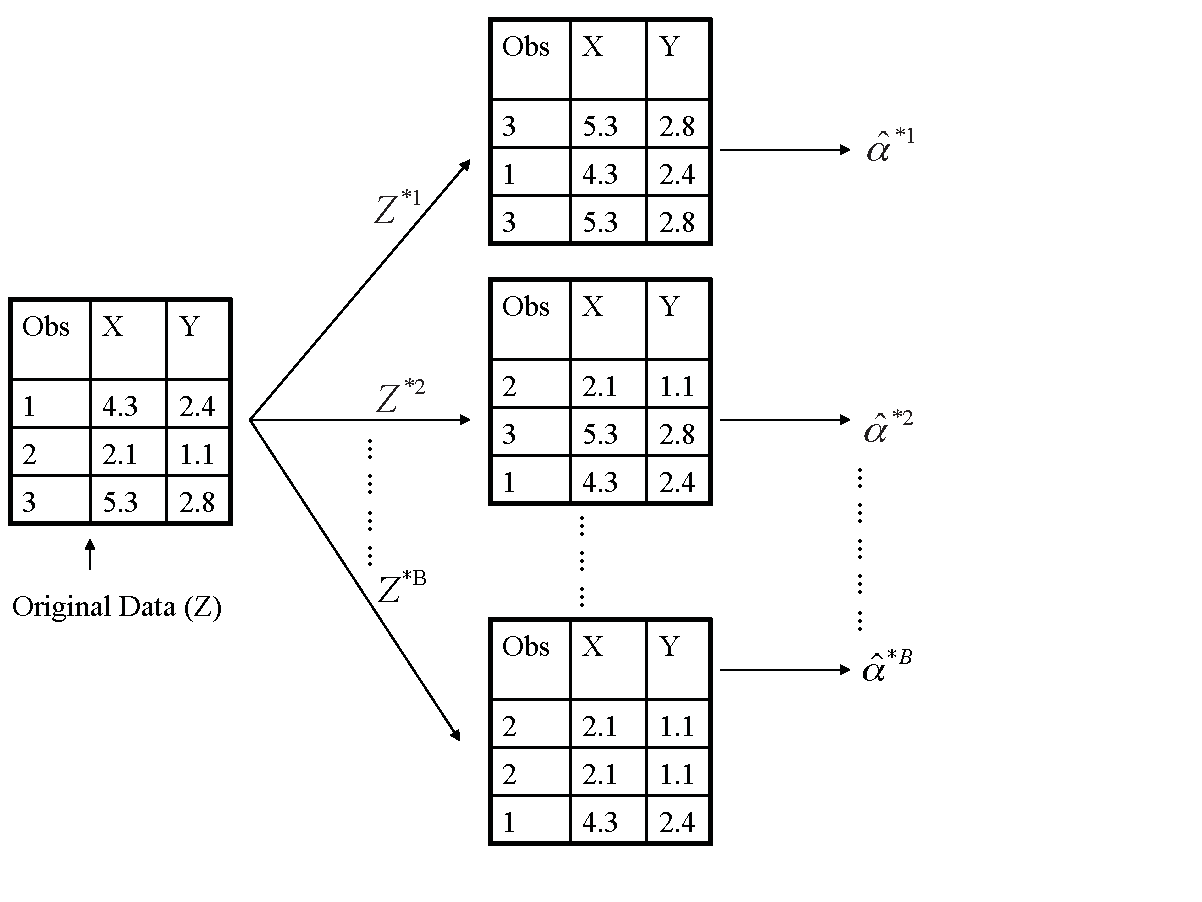
\includegraphics[width=0.95\textwidth,height=0.55\textheight,keepaspectratio]{5_11.pdf}
  \end{center}
  Each panel: histogram of $\hat\alpha$ over many bootstrap samples.
  The width of the histogram is the bootstrap SE.
  \islpsource{Figure 5.11}
\end{frame}

\begin{frame}{When the bootstrap works --- and when it fails}
  \begin{columns}[T]
    \begin{column}{0.48\textwidth}
      \begin{block}{Works for}
        \begin{itemize}
          \item Sample mean, variance, regression coefficients.
          \item Quantiles in the interior of the distribution.
          \item Correlation, $R^2$.
          \item Bagging in random forests.
        \end{itemize}
      \end{block}
    \end{column}
    \begin{column}{0.48\textwidth}
      \begin{alertblock}{Fails or misleads for}
        \begin{itemize}
          \item Extreme quantiles (max, min).
          \item Strongly dependent time series (use \emph{block}
                bootstrap).
          \item Hierarchical / clustered data (use cluster bootstrap).
          \item Small samples with discrete data.
        \end{itemize}
      \end{alertblock}
    \end{column}
  \end{columns}
  \begin{takeaway}
    Rule of thumb: the bootstrap is trustworthy when rows are roughly
    exchangeable and the statistic is smooth. Break either and you need
    a specialised variant (block, cluster, \dots).
  \end{takeaway}
\end{frame}

\begin{frame}{Exercise 5.5 --- Bootstrap Inclusion Probability [Math]}
  \begin{exercise}
    A bootstrap sample is drawn by sampling $n$ rows \emph{with
    replacement} from a data set of size $n$.
    \begin{enumerate}
      \item Show that the probability a specific observation is
            \emph{not} in a given bootstrap sample is
            $\bigl(1 - \tfrac1n\bigr)^n$.
      \item Hence write the probability that the observation \emph{is}
            included, and evaluate it for $n = 5$ and for $n = 1000$.
      \item What is the limiting inclusion probability as
            $n \to \infty$?
    \end{enumerate}
  \end{exercise}
\end{frame}

\begin{frame}{Solution --- Exercise 5.5 (1/2)}
  \begin{solutionbox}
    \textbf{(1) Probability of exclusion.}
    A single draw picks the given observation with probability
    $\tfrac1n$, hence misses it with probability $1 - \tfrac1n$.
    Because we sample \emph{with replacement}, the data set is restored
    before every draw, so the $n$ draws are independent and the $n$
    miss probabilities \emph{multiply}:
    \[
      P(\text{not included})
      = \underbrace{\bigl(1-\tfrac1n\bigr)\cdots\bigl(1-\tfrac1n\bigr)}_{n\ \text{draws}}
      = \Bigl(1 - \tfrac1n\Bigr)^n .
    \]
    \textbf{(2) Inclusion probability} (complement rule):
    $P(\text{included}) = 1 - \bigl(1 - \tfrac1n\bigr)^n$.
    \begin{itemize}
      \item $n = 5$: $\;1 - \tfrac15 = 0.8$, so
            $1 - (0.8)^5 = 1 - 0.3277 = 0.6723$.
      \item $n = 1000$: $\;1 - (0.999)^{1000} \approx 1 - 0.3677
            = 0.6323$.
    \end{itemize}
    \emph{Interpretation:} the inclusion probability \emph{falls} as $n$
    grows --- but only from $67\%$ to $63\%$, so it is already close to
    its limit for tiny samples.
  \end{solutionbox}
\end{frame}

\begin{frame}{Solution --- Exercise 5.5 (2/2)}
  \begin{solutionbox}
    \textbf{(3) Limit.}
    The standard limit $\lim_{n\to\infty}\bigl(1+\tfrac{x}{n}\bigr)^n
    = e^{x}$ with $x = -1$ gives
    $\bigl(1-\tfrac1n\bigr)^n \to e^{-1} \approx 0.3679$, hence
    \[
      P(\text{included}) \to 1 - e^{-1} \approx 1 - 0.3679 = 0.6321 .
    \]
    So each bootstrap sample contains, on average, about $63.2\%$ of the
    distinct original observations --- the famous $0.632$ figure. The
    remaining $\sim 36.8\%$ (the ``out-of-bag'' points) can serve as a
    built-in validation set, as used in bagging (Ch.~8).

    \emph{Common mistake:} concluding that a bootstrap sample is
    ``smaller'' than the data. It always contains exactly $n$ rows;
    $63.2\%$ is the expected fraction of \emph{distinct} originals ---
    the remaining slots are filled by duplicates.
  \end{solutionbox}
\end{frame}


\begin{frame}[fragile]{Extended Exercise 5.2 --- Bootstrap SE: Statistic and Coefficient [Python]}
  \begin{longexercise}
    Using \texttt{Portfolio} (columns \texttt{X},\texttt{Y}) and
    \texttt{Auto}, write Python that:
    \begin{enumerate}
      \item bootstraps ($B=1000$, resampling rows \emph{with
            replacement}) the minimum-variance allocation
            $\hat\alpha=\dfrac{\hat\sigma_Y^2-\hat\sigma_{XY}}
            {\hat\sigma_X^2+\hat\sigma_Y^2-2\hat\sigma_{XY}}$
            and reports the bootstrap SE and a $95\%$ \emph{percentile}
            interval;
      \item bootstraps the OLS slope of \texttt{mpg} on
            \texttt{horsepower} and compares the bootstrap SE with the
            textbook (formula-based) OLS standard error.
    \end{enumerate}
    Report the expected numbers and interpret the comparison in part~(2).
  \end{longexercise}
\end{frame}

\begin{frame}[fragile]{Solution --- Extended Exercise 5.2 (1/3)}
  \begin{lstlisting}
import numpy as np, pandas as pd
D = "../../ALL CSV FILES - 2nd Edition/"
Port = pd.read_csv(D+"Portfolio.csv")        # load Portfolio data
X, Y = Port["X"].values, Port["Y"].values    # two asset returns
def alpha(x, y):                             # min-variance allocation
    sx, sy = np.var(x, ddof=1), np.var(y, ddof=1)  # sample variances
    sxy = np.cov(x, y, ddof=1)[0, 1]         # sample covariance
    return (sy - sxy) / (sx + sy - 2*sxy)

rng = np.random.default_rng(0)               # reproducible RNG
n, B = len(X), 1000                          # B bootstrap replications
reps = np.empty(B)
for b in range(B):
    idx = rng.integers(0, n, n)         # sample WITH replacement
    reps[b] = alpha(X[idx], Y[idx])     # recompute alpha on resample
print(round(alpha(X, Y), 4), round(reps.std(ddof=1), 4),
      np.round(np.quantile(reps, [.025, .975]), 3))  # SE + 95% CI
  \end{lstlisting}
\end{frame}

\begin{frame}[fragile]{Solution --- Extended Exercise 5.2 (2/3)}
  \begin{lstlisting}
import statsmodels.api as sm
Auto = pd.read_csv(D+"Auto.csv", na_values="?").dropna()  # clean rows
hp  = Auto["horsepower"].values.astype(float)  # predictor
mpg = Auto["mpg"].values                       # response

ols = sm.OLS(mpg, sm.add_constant(hp)).fit()   # formula-based SE
print(round(ols.params[1], 4), round(ols.bse[1], 5))

m = len(hp); slopes = np.empty(1000)           # B = 1000 replications
for b in range(1000):
    idx = rng.integers(0, m, m)                # resample rows w/ replacement
    fit = sm.OLS(mpg[idx], sm.add_constant(hp[idx])).fit()  # refit OLS
    slopes[b] = fit.params[1]                  # store bootstrap slope
print(round(slopes.std(ddof=1), 5),            # bootstrap SE of slope
      np.round(np.quantile(slopes, [.025, .975]), 4))  # 95% interval
  \end{lstlisting}
\end{frame}

\begin{frame}{Solution --- Extended Exercise 5.2 (3/3)}
  \begin{solutionbox}[Expected numbers and interpretation]
    \textbf{Portfolio $\hat\alpha$.} $\hat\alpha\approx 0.576$, bootstrap
    $\widehat{\mathrm{SE}}\approx 0.091$, $95\%$ percentile interval
    $\approx[0.41,\,0.77]$. No closed-form SE exists, so the bootstrap is
    the natural tool (ISLP Section~5.2).

    \textbf{Auto slope.} OLS slope $\hat\beta_1\approx -0.158$ with
    formula SE $\approx 0.0064$; the bootstrap gives SE $\approx 0.0075$
    and interval $\approx[-0.173,\,-0.144]$.

    \textbf{Interpretation.} The two slope SEs are close, which
    \emph{validates} the bootstrap. Where they differ the bootstrap is
    often \emph{more trustworthy}: the formula SE assumes the linear
    model is correct with constant-variance errors, whereas the
    bootstrap assumes neither and picks up the mild
    non-linearity/heteroscedasticity in \texttt{Auto} --- hence the
    slightly larger bootstrap SE.

    \emph{Common mistake:} resampling \texttt{X} and \texttt{Y} as two
    \emph{independent} columns --- that destroys the covariance
    $\hat\sigma_{XY}$ that $\hat\alpha$ is built from. Always resample
    whole \emph{rows} (pairs), i.e.\ one shared index vector.
  \end{solutionbox}
\end{frame}

\begin{frame}{The bootstrap in action: the sampling distribution of $\hat\alpha$}
  \begin{center}
\includegraphics[width=0.88\textwidth,height=0.56\textheight,keepaspectratio]{ch05_x_bootstrap_alpha_hist.png}\end{center}
  \begin{takeaway}On \texttt{Portfolio.csv} the point estimate is $\hat\alpha = 0.576$; $B = 1000$ bootstrap resamples give $\widehat{\mathrm{SE}}(\hat\alpha) = 0.091$, so a rough $95\,\%$ range is $0.576 \pm 2(0.091) \approx [0.39,\,0.76]$ --- an uncertainty statement no closed-form formula supplies for $\alpha$.\end{takeaway}
\end{frame}

% ============================================================
\section{Python Lab}

\begin{frame}{Python lab --- run it live in the notebook}
  \begin{labnote}[Companion notebook: \texttt{chapter\_05\_lab.ipynb}]
    The code in this section is meant to be \textbf{demonstrated live}. Open the companion Jupyter notebook and run it cell by cell:
    \begin{itemize}
      \item the validation-set approach on the Auto data;
      \item $k$-fold cross-validation and LOOCV;
      \item the bootstrap.
    \end{itemize}
    Data loads via the \texttt{ISLP} package or the bundled CSV files; the notebook ends with hands-on exercises.
  \end{labnote}
\end{frame}


% ============================================================

\begin{frame}[fragile]{Validation set in scikit-learn}
  \begin{lstlisting}
from sklearn.model_selection import train_test_split
from sklearn.linear_model    import LinearRegression
from sklearn.metrics         import mean_squared_error
from ISLP import load_data

Auto = load_data("Auto")                     # load the Auto data
X = Auto[["horsepower"]].values; y = Auto["mpg"].values
Xtr,Xte,ytr,yte = train_test_split(X, y, test_size=0.5,
                                   random_state=1)  # one 50/50 split
mdl = LinearRegression().fit(Xtr, ytr)       # fit on training half only
mean_squared_error(yte, mdl.predict(Xte))    # validation-set MSE
  \end{lstlisting}
  Try changing \texttt{random\_state} and re-running --- the
  validation MSE will jump around noticeably.
\end{frame}

\begin{frame}[fragile]{$k$-fold cross-validation}
  \begin{lstlisting}
from sklearn.model_selection import KFold, cross_val_score
import numpy as np

cv = KFold(n_splits=10, shuffle=True, random_state=0)  # 10 folds
mse = -cross_val_score(LinearRegression(), X, y,  # 10 fits, one per fold
                       cv=cv, scoring="neg_mean_squared_error")
print(mse.mean(), mse.std())                 # CV estimate and spread
  \end{lstlisting}
  Always shuffle (unless time-ordered). The \texttt{neg\_} sign is a
  scikit-learn quirk: scores are always ``larger is better'', so MSE
  is negated.
\end{frame}

\begin{frame}[fragile]{Bootstrap of a regression coefficient}
  \begin{lstlisting}
import numpy as np
rng = np.random.default_rng(0)               # reproducible RNG

def boot_one(rng):
    idx = rng.integers(0, len(X), size=len(X))  # rows w/ replacement
    return LinearRegression().fit(X[idx], y[idx]).coef_[0]  # refit slope

B = 1000                                     # bootstrap replications
boots = np.array([boot_one(rng) for _ in range(B)])  # B slope replicates
print("SE:",  boots.std(ddof=1))             # bootstrap SE
print("95%:", np.quantile(boots, [0.025, 0.975]))  # percentile CI
  \end{lstlisting}
\end{frame}

\begin{frame}[fragile]{Exercise 5.6 --- Bootstrap SE of the Portfolio $\alpha$ [Python]}
  \begin{exercise}
    The Portfolio data has returns \texttt{X} and \texttt{Y}. The
    minimum-variance allocation is
    \[
      \hat\alpha =
      \frac{\hat\sigma_Y^2 - \hat\sigma_{XY}}
           {\hat\sigma_X^2 + \hat\sigma_Y^2 - 2\hat\sigma_{XY}} .
    \]
    Write Python that (i) computes $\hat\alpha$ on the full sample and
    (ii) estimates its standard error with $B = 1000$ bootstrap
    resamples. Report the expected result.
  \end{exercise}
\end{frame}

\begin{frame}[fragile]{Solution --- Exercise 5.6 (1/2)}
  \begin{solutionbox}[Method --- why the bootstrap is the right tool]
    $\hat\alpha$ is a nonlinear \emph{ratio} of variances and a
    covariance, so no textbook SE formula applies. Bootstrap plug-in
    principle: treat the sample as the population, draw $n$ rows
    \emph{with replacement} (keeping each $(X_i, Y_i)$ pair together),
    recompute $\hat\alpha$ on every resample, and report the sample SD
    of the $B$ replicates as $\widehat{\mathrm{SE}}(\hat\alpha)$.
  \end{solutionbox}
  \begin{lstlisting}
import numpy as np, pandas as pd
Port = pd.read_csv("../../ALL CSV FILES - 2nd Edition/Portfolio.csv")
X = Port["X"].values; Y = Port["Y"].values   # two asset returns

def alpha(x, y):                             # min-variance allocation
    sx, sy = np.var(x, ddof=1), np.var(y, ddof=1)  # sample variances
    sxy = np.cov(x, y, ddof=1)[0, 1]         # sample covariance
    return (sy - sxy) / (sx + sy - 2*sxy)

a_hat = alpha(X, Y)              # point estimate
  \end{lstlisting}
\end{frame}

\begin{frame}[fragile]{Solution --- Exercise 5.6 (2/2)}
  \begin{lstlisting}
rng = np.random.default_rng(0)               # reproducible RNG
n, B = len(X), 1000                          # B bootstrap replications
reps = np.empty(B)
for b in range(B):
    idx = rng.integers(0, n, size=n)   # sample with replacement
    reps[b] = alpha(X[idx], Y[idx])    # recompute alpha on resample

print("alpha_hat:", round(a_hat, 4))
print("bootstrap SE:", round(reps.std(ddof=1), 4))  # SD of replicates
  \end{lstlisting}
  \begin{solutionbox}[Expected result]
    You should obtain $\hat\alpha \approx 0.58$ and a bootstrap standard
    error of roughly $\widehat{\mathrm{SE}}(\hat\alpha) \approx 0.09$
    (matching ISLP Section~5.2). Interpretation: across resamples the
    estimated optimal allocation to asset $X$ varies by about $\pm 0.09$,
    which quantifies the uncertainty in $\hat\alpha$ with no closed-form
    formula required.

    \emph{Common mistake:} drawing separate index vectors for \texttt{X}
    and \texttt{Y} --- that breaks the $X$--$Y$ covariance the statistic
    depends on. One shared \texttt{idx} keeps the pairs intact.
  \end{solutionbox}
\end{frame}


\begin{frame}{Extended Exercise 5.3 --- Leak-Free CV for Tuning and Evaluation [Integrative]}
  \begin{longexercise}
    You must (a) choose a tuning parameter --- say the polynomial degree
    $d$ (or the KNN neighbourhood size $K$) --- \emph{and} (b) report an
    honest estimate of the final model's test error.
    \begin{enumerate}
      \item A colleague standardises all predictors and selects the best
            $d$ features on the \emph{full} data set, \emph{then} runs
            10-fold CV. Explain precisely why the resulting error
            estimate is optimistically biased (data leakage).
      \item Design the \emph{correct} procedure. Where must scaling,
            feature selection, and the $d$/$K$ choice happen relative to
            the CV split?
      \item Sketch a \emph{nested} CV that both tunes $d$/$K$ and gives an
            unbiased test-error estimate. What does each loop do?
    \end{enumerate}
  \end{longexercise}
\end{frame}

\begin{frame}{Solution --- Extended Exercise 5.3 (1/3)}
  \begin{solutionbox}[Why full-data preprocessing leaks]
    \textbf{(1) The leak.} Cross-validation is honest only if each
    validation fold is treated exactly like genuinely unseen data. If you
    standardise or select features using \emph{all} $n$ rows first, then
    every validation fold has already influenced
    \begin{itemize}
      \item the scaling constants (means/SDs use the fold's own rows), and
      \item which features are kept (the choice saw the fold's response).
    \end{itemize}
    The model is then scored on data that helped build it, so the CV
    error \emph{underestimates} the true test error --- sometimes
    dramatically when $p$ is large and selection is aggressive. The fold
    is no longer ``held out''.
  \end{solutionbox}
\end{frame}

\begin{frame}[fragile]{Solution --- Extended Exercise 5.3 (2/3)}
  \begin{solutionbox}[Correct procedure: everything inside the split]
    Fit \emph{all} data-dependent steps --- scaling, feature selection,
    and the $d$/$K$ choice --- \emph{inside} each training fold only. A
    \texttt{Pipeline} makes this automatic: the search re-fits every step
    on each fold's training part.
  \end{solutionbox}
  \begin{lstlisting}
from sklearn.pipeline import Pipeline
from sklearn.preprocessing import StandardScaler, PolynomialFeatures
from sklearn.linear_model import LinearRegression
from sklearn.model_selection import GridSearchCV, KFold

pipe = Pipeline([("scale", StandardScaler()),  # scaling INSIDE each fold
                 ("poly",  PolynomialFeatures()),  # degree = tuning param
                 ("lm",    LinearRegression())])
inner  = KFold(10, shuffle=True, random_state=0)  # inner tuning loop
search = GridSearchCV(pipe, {"poly__degree": [1, 2, 3, 4, 5]},  # d grid
                      cv=inner, scoring="neg_mean_squared_error")
  \end{lstlisting}
\end{frame}

\begin{frame}[fragile]{Solution --- Extended Exercise 5.3 (3/3)}
  \begin{lstlisting}
from sklearn.model_selection import cross_val_score
outer = KFold(5, shuffle=True, random_state=1)  # outer evaluation loop
test_err = -cross_val_score(search, X, y, cv=outer,  # nested CV
                            scoring="neg_mean_squared_error")
print("chosen degree:", search.fit(X, y).best_params_)  # tuned d
print("unbiased test MSE:", test_err.mean(), "+/-", test_err.std())
  \end{lstlisting}
  \begin{solutionbox}[Nested CV --- two loops and two jobs]
    \textbf{(3)} The \emph{inner} loop (inside \texttt{GridSearchCV})
    selects $d$/$K$ using only each outer-training part. The \emph{outer}
    loop scores the whole tuning procedure on data it never touched,
    giving an \emph{unbiased} test-error estimate. Tuning and evaluation
    use disjoint data, so neither contaminates the other.
  \end{solutionbox}
\end{frame}

% ============================================================
\section{Summary}
% ============================================================

\begin{frame}{Chapter 5 in one slide}
  \begin{block}{What we accomplished}
    Acquired the most important practical skill in statistical
    learning: estimating test error and uncertainty without an oracle
    test set.
  \end{block}
  \begin{itemize}
    \item Validation set, LOOCV, $k$-fold CV --- three estimators of
          test error.
    \item Bias--variance trade-off \emph{within} the estimator itself.
    \item The bootstrap for standard errors and confidence intervals.
    \item Common pitfalls: leakage, time-series CV, grouped data.
  \end{itemize}
\end{frame}

\begin{frame}{Vocabulary checklist}
  \footnotesize
  \begin{tabular}{ll}
    \toprule
    \textbf{Term} & \textbf{Meaning} \\
    \midrule
    Validation set & Single random hold-out split \\
    LOOCV & Leave-one-out CV ($k = n$) \\
    $k$-fold CV & Average of $k$ disjoint hold-outs \\
    Bootstrap & Resample with replacement, $B$ times \\
    Standard error (SE) & SD of an estimator across samples \\
    Information leakage & Test info bleeding into training pipeline \\
    Nested CV & CV for tuning, second CV for evaluation \\
    Block bootstrap & For time series \\
    Cluster bootstrap & For grouped data \\
    \bottomrule
  \end{tabular}
\end{frame}

\begin{frame}{Key formulas at a glance}
  \begin{block}{$k$-fold and LOOCV estimates}
    \[
      \mathrm{CV}_{(k)} = \tfrac{1}{k}\sum_{j=1}^{k}\mathrm{MSE}_j,
      \qquad
      \mathrm{CV}_{(n)} = \tfrac{1}{n}\sum_{i=1}^{n}\bigl(\tfrac{y_i - \hat y_i}{1 - h_i}\bigr)^2 \text{ (OLS).}
    \]
  \end{block}
  \begin{block}{Bootstrap SE}
    \[
      \widehat{\mathrm{SE}}(\hat\alpha) =
        \sqrt{\tfrac{1}{B-1}\sum_{b=1}^{B}(\hat\alpha^{*b} - \bar\alpha^*)^2}.
    \]
  \end{block}
\end{frame}

\begin{frame}{Methods comparison}
  \footnotesize
  \begin{tabular}{lll}
    \toprule
    \textbf{Procedure} & \textbf{Bias} & \textbf{Variance / Cost} \\
    \midrule
    Single validation set & Upward & High variance \\
    LOOCV & Lowest & Highest variance, $n$ fits \\
    5-fold CV & Slightly upward & Moderate variance, 5 fits \\
    10-fold CV & Smaller bias than 5-fold & Moderate variance \\
    Bootstrap & Estimates SE, not test error & $B$ fits \\
    \bottomrule
  \end{tabular}
\end{frame}

\begin{frame}{Decision rules of thumb}
  \begin{itemize}
    \item For tuning a hyperparameter: 5- or 10-fold CV.
    \item For final evaluation: external held-out set or nested CV.
    \item For SEs and CIs: bootstrap (or theory if available).
    \item For time series: rolling-origin CV (\emph{never} random
          folds).
    \item For grouped data: split at the group level.
    \item Always fit \emph{all} preprocessing inside the CV loop.
  \end{itemize}
\end{frame}

\begin{frame}{Common pitfalls}
  \begin{alertblock}{Don't}
    \begin{enumerate}
      \item Standardise / impute / select features on the full data
            \emph{before} CV.
      \item Use random folds for time series.
      \item Optimise tuning parameters on the same fold you score
            them on.
      \item Confuse the bootstrap with cross-validation --- they
            answer different questions.
      \item Use the bootstrap for extreme quantiles or under strong
            dependence.
      \item Report a single CV score without an estimate of its
            variability.
    \end{enumerate}
  \end{alertblock}
\end{frame}

\begin{frame}{Connections to the rest of the course}
  \begin{itemize}
    \item Ch.~6: cross-validation chooses $\lambda$ in ridge / lasso.
    \item Ch.~7: cross-validation chooses spline df and LOESS span.
    \item Ch.~8: bagging is the bootstrap; OOB error is built-in CV.
    \item Ch.~10: tune learning rate, dropout via CV.
    \item Ch.~13: resampling-based $p$-values and FDR-control
          procedures.
  \end{itemize}
\end{frame}

\begin{frame}{Self-check questions}
  \begin{enumerate}
    \item Why does the validation-set estimate have such high variance?
    \item Show that 5-fold CV has lower variance than LOOCV.
    \item How would you cross-validate a model on a time series?
    \item Describe a scenario in which the bootstrap estimate of SE is
          wrong.
    \item Outline a nested-CV procedure for unbiased evaluation while
          tuning a hyperparameter.
    \item For OLS, derive the LOOCV shortcut formula using leverage.
  \end{enumerate}
\end{frame}

\begin{frame}{Five things to remember}
  \begin{enumerate}
    \item Resampling lets us estimate test error and uncertainty
          without a separate test set.
    \item Validation set: simple but variable.
    \item LOOCV: low bias, high variance, computational shortcuts for
          OLS.
    \item $k$-fold ($k = 5$ or $10$): the workhorse compromise.
    \item Bootstrap: resample with replacement to estimate SEs and
          CIs.
  \end{enumerate}
\end{frame}

\begin{frame}{What's next}
  Chapter 6: \emph{Linear Model Selection and Regularisation}.
  \begin{itemize}
    \item Subset selection.
    \item Ridge regression and the lasso.
    \item Dimension reduction: PCR and PLS.
    \item How to use cross-validation to pick tuning parameters.
  \end{itemize}
\end{frame}

\end{document}
